	\newpage
\section{Podręcznik użytkownika}  %6
%Opis jak używać programu. Mogą być z zrzut ekranu razem z opisem. 

\subsection{Czym jest BikeApp?} %6.1

BikeApp jest aplikacją stworzoną dla rowerzystów wszelkiego rodzaju, od osób jeżdżących rekreacyjnie, przez turystów aż po zawodowych kolarzy (rysunek 6.1). Pozwala na zapisanie w pamięci telefonu różnych danych, które mogą być mu potrzebne, takich jak często odbywane trasy oraz dane pomiarowe. Oferuje przy tym prostą obsługę tych udogodnień oraz możliwość spersonalizowania ustawień.\\
\\
Niniejsza instrukcja zawiera informacje odnośnie korzystania z aplikacji, a w szczególności - komponentów, na które się ona składa. Jedna z podsekcji poświęcona została także znanym problemom, na które użytkownik może natrafić, korzystając z BikeApp.\\

\begin{figure}[!htb]
	\begin{center}
		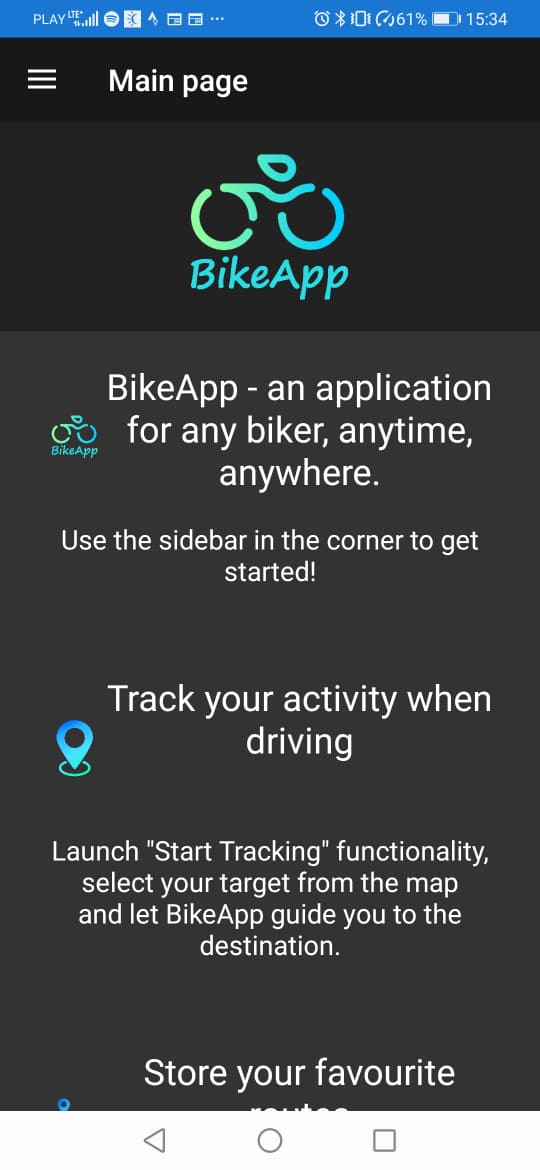
\includegraphics[width=6cm]{rys/instructions-mainpage.jpg}
		\caption{BikeApp - strona główna}
		\label{rys:BikeApp - strona główna}
	\end{center}
\end{figure}

\subsection{Dostęp do menu głównego oraz spis podstron} %6.2
Aplikacja BikeApp podzielona jest na podstrony, zaś dostęp do nich możliwy jest za pośrednictwem menu głównego.\\
\\
Menu główne jest otwierane przy użyciu znajdującej się w lewym górnym rogu ekranu ikony trzech poziomych linii. Jżeli zamiast niej widoczna jest strzałka, wówczas oznacza ona cofnięcie się do poprzedniej podstrony i należy ją wybierać i cofać się aż do pojawienia się ikony otwarcia menu głównego.\\
\\
Wybranie opcji na menu głównym (rysunek 6.2) spowoduje otwarcie właściwej podstrony poświęconej danej funkcji. Tematy obsługi poszczegónych podstron oraz opisu funkcji rozwinięto w dalszych podrozdziałach.

\begin{figure}[!htb]
	\begin{center}
		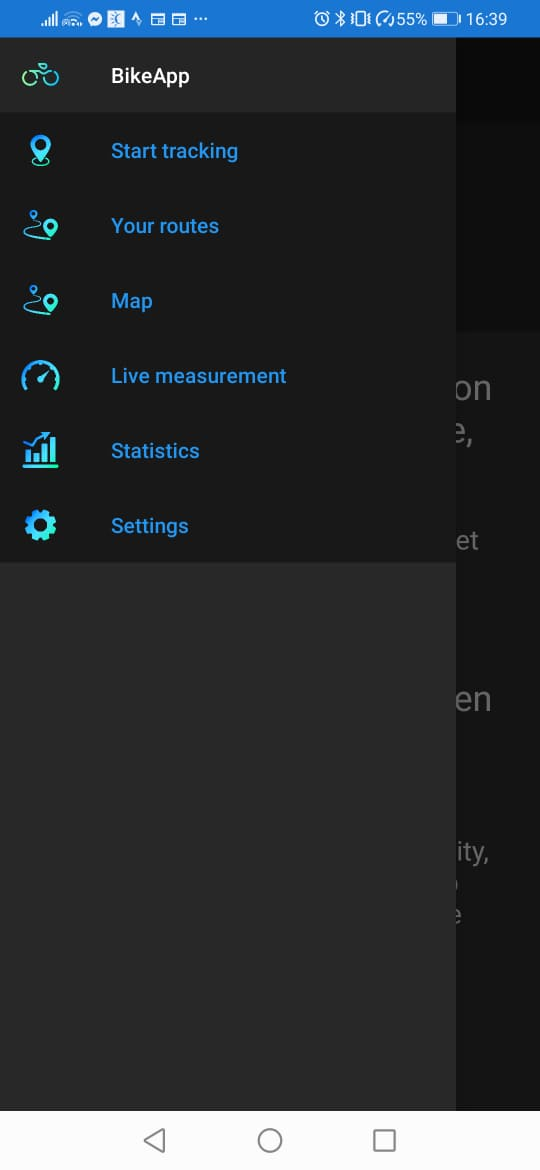
\includegraphics[width=6cm]{rys/instructions-menu.jpg}
		\caption{BikeApp - menu główne}
		\label{rys:BikeApp - menu główna}
	\end{center}
\end{figure}

\subsection{Mechanizm śledzenia trasy} %6.3
Tryb śledzenia trasy pozwala na zapisanie ścieżki, którą użytkownik przebędzie w trakcie jego działania. Powstała w ten sposób trasa może następnie zostać wyświetlona na mapie bądź zapisana w pamięci telefonu w celu późniejszego przeglądania.\\
\\
Aby uruchomić podstronę śledzenia trasy, należy rozwinąć menu główne i wybrać opcję ``Start Tracking''.\\
\\
Tryb śledzenia trasy jest uruchamiany poprzez wybranie przycisku ``Start tracking'' na podstronie (rysunek 6.3). Jego włączenie potwierdzi stosowny wyskakujący komunikat. Ponowne użycie tego samego przycisku zatrzymuje działanie trybu śledzenia trasy, a następnie wyświetla monit o nadanie trasie nazwy, po czym zostaje ona zapisana przez aplikację.\\
\\
W trakcie śledzenia trasy możliwe jest wykonywanie innych czynności na telefonie, w tym zamknięcie okna aplikacji i wyjście do ekranu głównego systemu telefonu.

\begin{figure}[!htb]
	\begin{center}
		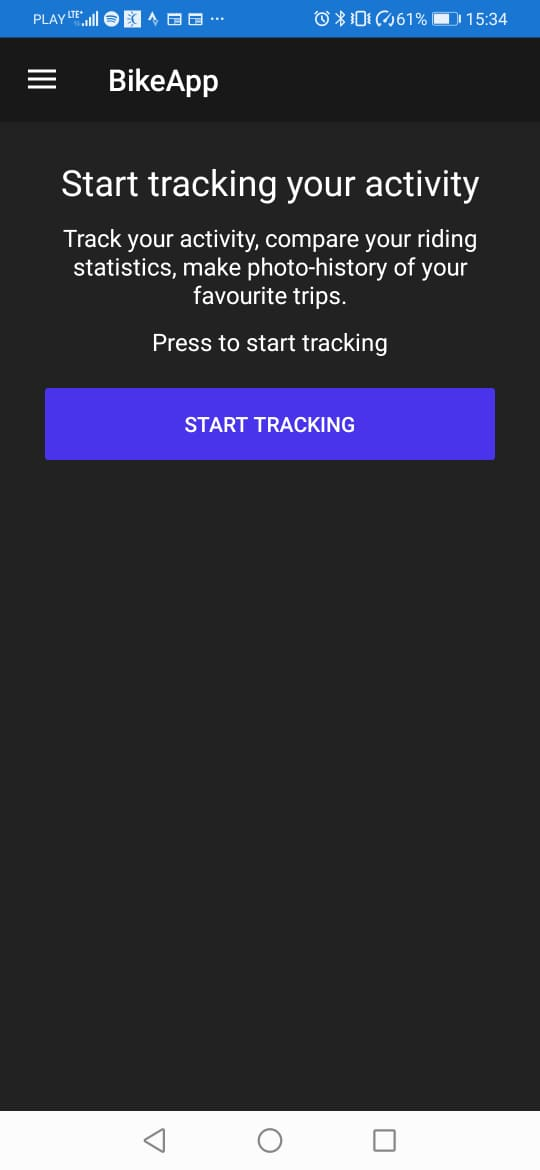
\includegraphics[width=6cm]{rys/instructions-tracking.jpg}
		\caption{BikeApp - podstrona śledzenia trasy}
		\label{rys:BikeApp - podstrona śledzenia trasy}
	\end{center}
\end{figure}

\subsection{Zarządzanie zapisanymi trasami} %6.4
Po zakończeniu śledzenia danej trasy, jest ona zapisywana pod nazwą wskazaną przez uzytkownika. Lista tras oraz parametry każdej z nich dostępne są z poziomu specjalnej podstrony.\\
\\
Aby obejrzeć zapisane trasy, należy rozwinąć menu główne i wybrać opcję ``Your Routes''.\\
\\
Każda pozycja na liście może zostać zaznaczona, co przeniesie użytkownika do ekranu z informacjami na temat wybranej trasy (rysunek 6.4). Aby powrócić do ekranu ze spisem zapisanych tras, należy uzyć strzałki znajdującej się w lewym górnym rogu. Działanie przycisku ``Display on Map'' opisano w podrozdziale ``Wyświetlanie trasy na mapie'' niniejszej instrukcji.

\begin{figure}[!htb]
	\begin{center}
		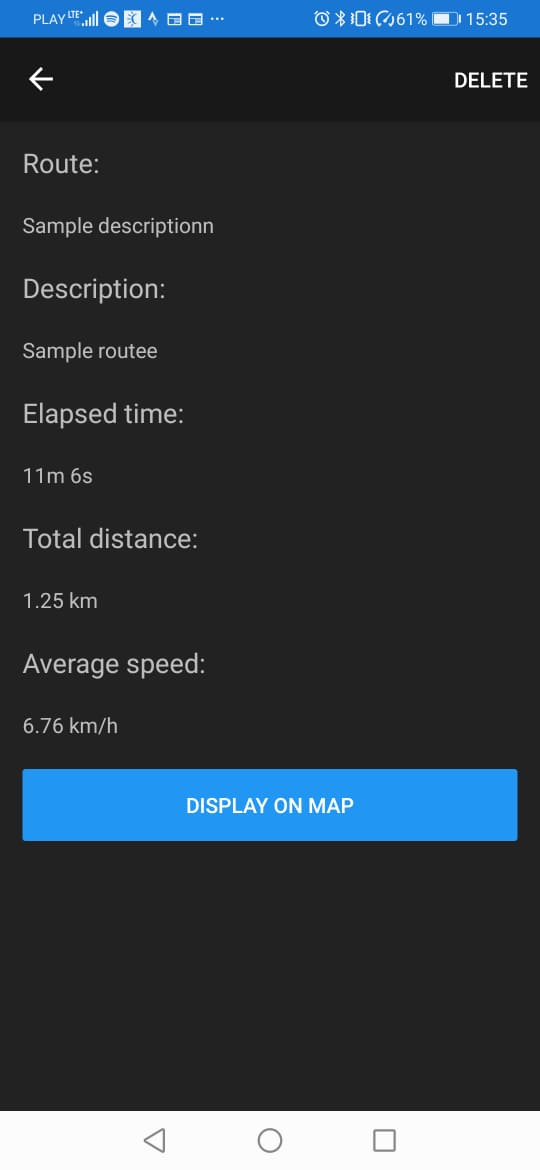
\includegraphics[width=6cm]{rys/instructions-route-details.jpg}
		\caption{BikeApp - szczegóły trasy}
		\label{rys:BikeApp - szczegóły trasy}
	\end{center}
\end{figure}

\subsection{Wyświetlanie trasy na mapie} %6.5
BikeApp zawiera podstronę z Mapą Google, dzięki której zapisane w pamięci telefonu trasy można obejrzeć w trybie graficznym. Będzie ona widoczna jako seria punktów połączonych prostymi liniami.\\
\\
Istnieją dwa sposoby na otwarcie Mapy Google wewnątrz aplikacji. Pierwszym jest wybranie opcji ``Map'' z menu głównego, drugim zaś - uruchomienie podstrony z listą tras, wybranie trasy oraz użycie przycisku ``Display on Map''. W przypadku sukcesu, widok będzie podobny, jak na rysunku 6.5.\\
\\
Przesuwanie oraz regulacja przybliżenia widoku na mapę odbywają się w sposób standardowy dla Map Google uruchamianych na urządzeniach mobilnych. Aplikacja nakłada również na mapę linie reprezentujące wybraną trasę.

\begin{figure}[!htb]
	\begin{center}
		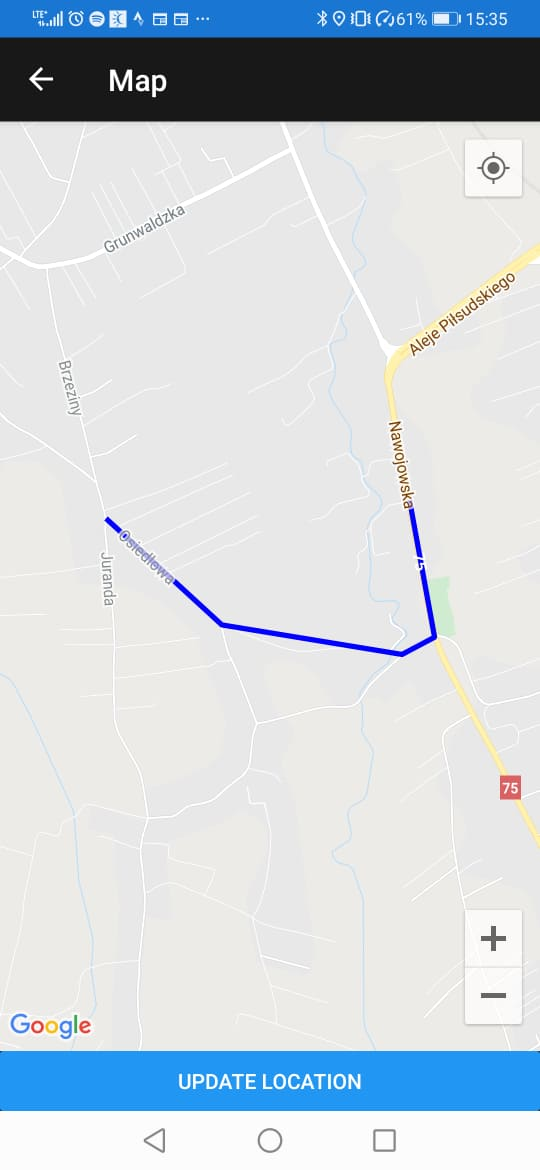
\includegraphics[width=6cm]{rys/instructions-map.jpg}
		\caption{BikeApp - Mapa Google}
		\label{rys:BikeApp - Mapa Google}
	\end{center}
\end{figure}

\subsection{Przeglądanie danych pomiarowych} %6.6
Aplikacja BikeApp może dokonywać pomiarów w trakcie jazdy. Mierzone są takie parametry jak kąty nachylenia urządzenia, przeciążenia oraz wystąpienia skoków przeciążeń, wynikających przykładowo z natrafienia na przeszkodę. Dane te mogą być wyświetlane na bieżąco bądź zbierane i przechowywane jako statystyki użytkownika.

\subsubsection{Dane chwilowe} %6.6.1
Aby uzyskać dostęp do danych wyświetlanych w momencie pobrania, należy z poziomu menu głównego wybrać pozycję ``Live measurement''. Użytkownikowi ukaże się podstrona wyglądająca tak, jak na rysunku 6.6.\\
\\
Pomiary danych są domyślnie zatrzymane po uruchomieniu aplikacji. Można je rozpocząć, korzystając z przełącznika odpowiadającego pozycji ``Accelerometer''. Poniżej przełączników będą widoczne zmierzone przez aplikację wartości.\\
\\
Drugi przełącznik, opisany nazwą ``Shake detection'', obsługuje wykrywanie skoków przeciążenia. Gdy jest ono aktywne, każdy moment, w którym pomiar przeciążenia wykaże odpowiednio wysoką wartość, będzie odnotowywany poprzez wyskakujące okienko. Wykrywania skoków przeciążenia nie można uruchomić, jeśli wyłączone jest także pobieranie danych chwilowych.

\begin{figure}[!htb]
	\begin{center}
		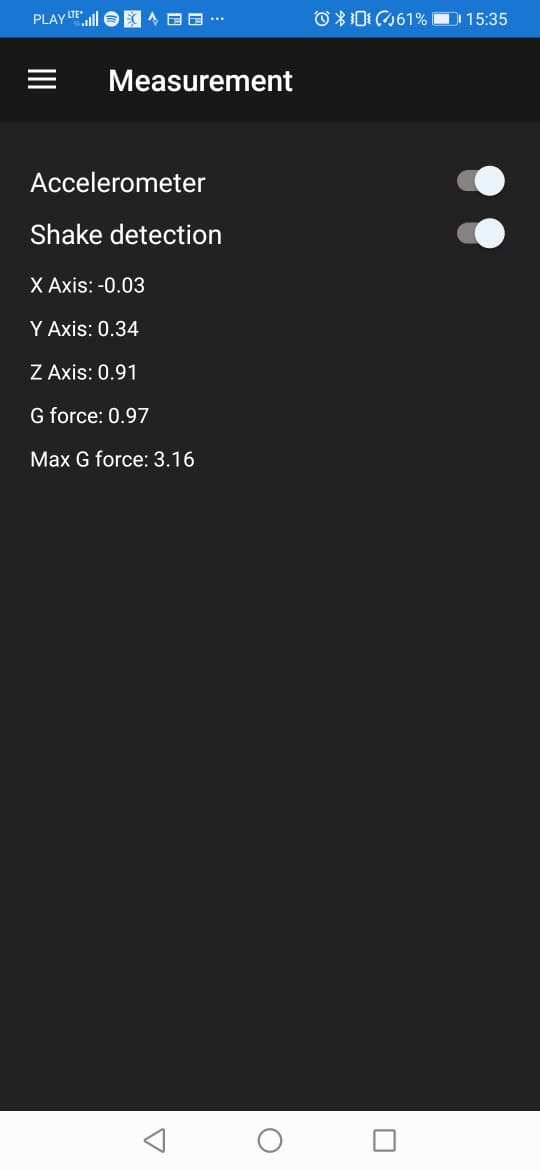
\includegraphics[width=6cm]{rys/instructions-measurement.jpg}
		\caption{BikeApp - Pomiary chwilowe}
		\label{rys:BikeApp - Pomiary chwilowe}
	\end{center}
\end{figure}

\subsubsection{Dane gromadzone w czasie (statystyki)} %6.6.1
Aby zobaczyć dane zbierane w dłuższym przedziale czasu, należy otworzyć menu główne i wybrać opcję ``Statistics''.\\
\\
Podstrona statystyk (rysunek 6.7) przedstawia różne rodzaje danych zgromadzonych przez aplikację w czasie, gdy tryb śledzenia trasy był aktywny. Obejmuje zarówno informacje o wartościach minimalnych i maksymalnych, jak również średnich.

\begin{figure}[!htb]
	\begin{center}
		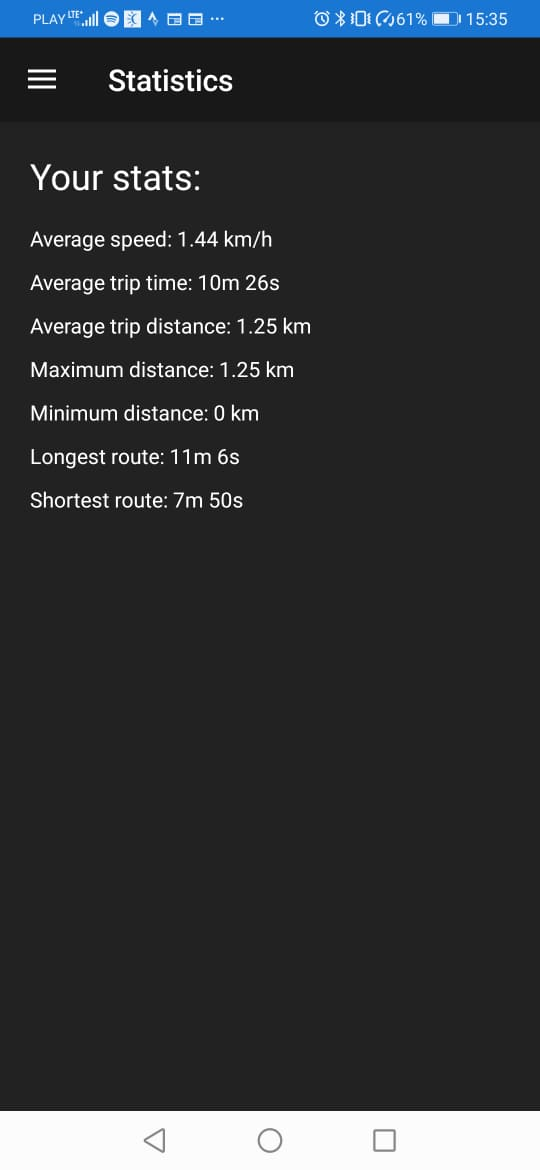
\includegraphics[width=6cm]{rys/instructions-stats.jpg}
		\caption{BikeApp - Podstrona statystyk}
		\label{rys:BikeApp - Podstrona statystyk}
	\end{center}
\end{figure}

\subsection{Dostosowanie ustawień} %6.7
Ustawienia aplikacji dostępne są za pośrednictwem menu głównego. Po jego otwarciu należy wybrać pozycję ``Settings''.\\
\\
Poszczególne opcje dostępne są w postaci przełączników, które można aktywować lub deaktywować poprzez ich użycie. Każda zmiana ustawień zatwierdzana jest natychmiast po jej wystąpieniu.

\subsection{Częste problemy i błędy} %6.8
Lorem ipsum...


